\subsection{MSVC: x86}

Il seguente e' l'output assembly ottenuto con MSVC 2010:

\lstinputlisting{patterns/04_scanf/3_checking_retval/ex3_MSVC_x86.asm}

\myindex{x86!\Registers!EAX}
La funzione chiamante (\gls{caller}) \main necessita di ottenere il risultato della funzione chiamata (\gls{callee}), 
e pertanto quest'ultima lo restituisce nel registro \EAX register.

\myindex{x86!\Instructions!CMP}
Il controllo viene eseguito con l'aiuto dell'istruzione \TT{CMP EAX, 1} (\IT{CoMPare}). In altre parole, confrontiamo il valore nel registro \EAX con 1.

\myindex{x86!\Instructions!JNE}
U jump condizionale \JNE segue l'istruzione \CMP. \JNE sta per \IT{Jump if Not Equal}.

Quindi, se il valore nel registro \EAX non e' uguale a 1, la \ac{CPU} passera' l'esecuzione all'indirizzo specificato nell'operando di \JNE, nel nostro caso \TT{\$LN2@main}.
Passare il controllo a questo indirizzo risulta nel fatto che la \ac{CPU} eseguira' la funzione \printf con l'argomento \TT{What you entered? Huh?}.
Ma se tutto va bene, il salto condizionale non viene effettuato, e viene eseguita un'altra chiamata a \printf con due argomenti: \TT{'You entered \%d...'} e il valore di \TT{x}.

\myindex{x86!\Instructions!XOR}
\myindex{\CLanguageElements!return}
Poiche' in questo caso la saconda \printf non deve essere eseguita, c'e' un jump non condizionale (unconditional jump) \JMP che la precede. 
Questo passa il controllo al punto dopo la seconda \printf e prima dell'istruzione \TT{XOR EAX, EAX}, che implementa \TT{return 0}.

% FIXME internal \ref{} to x86 flags instead of wikipedia
\myindex{x86!\Registers!\Flags}
Possiamo quindi dire che il confronto di valori e' \IT{solitamente} implementato con una coppia di istruzioni \CMP/\Jcc, dove \IT{cc} e' un \IT{condition code}.
\CMP confronta due valori e imposta i flag del processore \footnote{x86 flags, vedere anche: \href{http://go.yurichev.com/17120}{wikipedia}.}.
\Jcc controlla questi flag e decide se passare o meno il controllo all'indirizzo specificato.

\myindex{x86!\Instructions!CMP}
\myindex{x86!\Instructions!SUB}
\myindex{x86!\Instructions!JNE}
\myindex{x86!\Registers!ZF}
\label{CMPandSUB}
Puo' sembrare un paradosso, ma l'istruzione \CMP e' in effetti una \SUB (subtract).
Tutte le istruzioni aritmetiche settano i flag del processore, non solo \CMP.
Se confrontiamo 1 e 1, $1-1$ e' 0 e quindi il flag \ZF sarebbe impostato a 1 (significando che l'ultimo risultato era 0).
In nessun'altra circostanza il flag \ZF puo' essere impostato, eccetto il caso in cui gli operandi sono uguali.
\JNE controlla soltanto il flag \ZF e salta se e solo se il flag non e' settato.  \JNE e' infatti un sinonimo di \JNZ (\IT{Jump if Not Zero}).
L'assembler traduce entrambe le istruzioni \JNE e \JNZ nello stesso opcode.
Quindi l'istruzione \CMP puo' essere sostituita dall'istruzione \SUB e quasi tutto funzionera', con la differenza che \SUB altera il valore del primo operando.
\CMP e' uguale a \IT{SUB senza salvare il risultato, ma settando i flag}.

\subsection{MSVC: x86: IDA}

\myindex{IDA}
E' arrivato il momento di avviare \IDA. A proposito, per i principianti e' buona norma usare l'opzione \TT{/MD} in MSVC, che significa che tutte le funzioni
standard non saranno linkate dentro il file eseguibile, ma importate dal file \TT{MSVCR*.DLL}.
In questo modo sara' piu' facile vedere quali funzioni standard sono usate, e dove.

Quando si analizza il codice con \IDA, e' sempre molto utile lasciare note per se stessi (e per gli altri, nel caso in cui si lavori in gruppo).
Per esempio, analizzando questo esempio, notiamo che 
\TT{JNZ} sara' innescato in caso di errore.
E' possibile muovere il cursore fino alla label, premere \q{n} e rinominarla in \q{errore}.
Creare un'altra label ---in \q{exit}.
Ecco il mio risultato:

\lstinputlisting{patterns/04_scanf/3_checking_retval/ex3.lst}

Adesso e' leggermente piu' facile capire il codice.
Non e' comunque una buona idea commentare ogni istruzione!

% FIXME draw button?
Si possono anche nascondere (collapse) parti di una funzione in \IDA.
Per farlo, selezionare il blocco e premere \q{--} sul tastierino numerico, inserendo il testo da visualizzare al posto del blocco di codice.

Nascondiamo due blocchi e diamogli un nome:

\lstinputlisting{patterns/04_scanf/3_checking_retval/ex3_2.lst}

% FIXME draw button?
Per espandere dei blocchi nascosti, premere \q{+} sul tastierino numerico.

\clearpage
Premendo \q{spazio}, possiamo vedere come \IDA rappresenta una funzione in forma di grafo:

\begin{figure}[H]
\centering
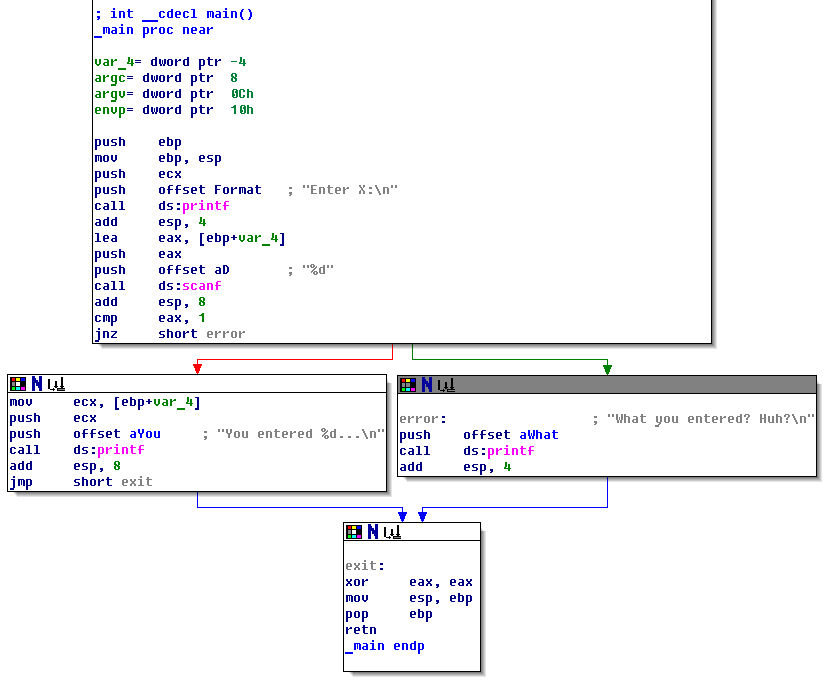
\includegraphics[scale=\FigScale]{patterns/04_scanf/3_checking_retval/IDA.png}
\caption{Graph mode in IDA}
\label{fig:ex3_IDA_1}
\end{figure}

Ci sono due frecce dopo ogni jump condizionale: verde e rossa.
La freccia verde punta al blocco che viene eseguito se il jump e' innescato, la rossa nel caso opposto.

\clearpage
Anche in questa modalita' e' possibile "chiudere" i nodi e dargli un'etichetta (\q{group nodes}).
Facciamolo per 3 blocchi:

\begin{figure}[H]
\centering
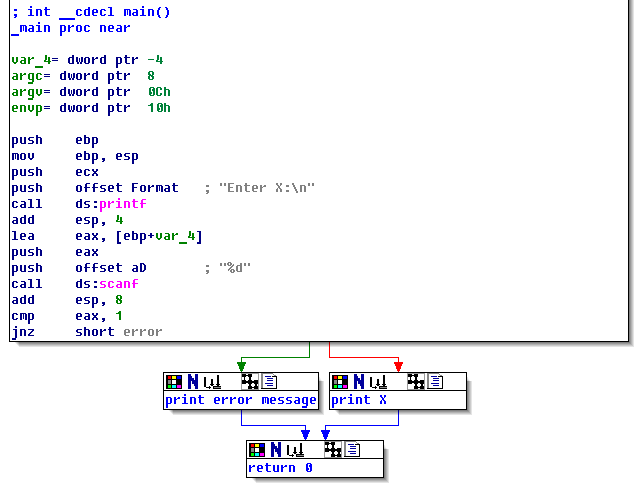
\includegraphics[scale=\FigScale]{patterns/04_scanf/3_checking_retval/IDA2.png}
\caption{Graph mode in IDA with 3 nodes folded}
\label{fig:ex3_IDA_2}
\end{figure}

Come si puo' vedere questa funzione e' molto utile.
Si puo' dire che una buona parte del lavoro di un reverse engineer (cosi' come di altri tipi di ricercatori) e' rappresentata dalla riduzione della quantita' di informazioni da trattare.

\clearpage
\subsectionold{MSVC: x86 + \olly}

Proviamo ad hackerare il nostro programma in \olly, forzandolo a pensare che \scanf funzioni sempre senza errori.
Quando l'indirizzo di una variabile locale e' passato a \scanf, la variabile inizialmente contiene un valore random inutile, in questo caso \TT{0x6E494714}:

\begin{figure}[H]
\centering
\myincludegraphics{patterns/04_scanf/3_checking_retval/olly_1.png}
\caption{\olly: passing variable address into \scanf}
\label{fig:scanf_ex3_olly_1}
\end{figure}

\clearpage
Quando \scanf viene eseguita, immettiamo nella console qualcosa di diverso da un numero, come \q{asdasd}.
\scanf finisce con 0 in \EAX, indicante che un errore si e' verificato:

\begin{figure}[H]
\centering
\myincludegraphics{patterns/04_scanf/3_checking_retval/olly_2.png}
\caption{\olly: \scanf returning error}
\label{fig:scanf_ex3_olly_2}
\end{figure}

Possiamo anche controllare la variabile locale nello stack e notare che non e' stata modificata.
Infatti cosa avrebbe potuto scrivere \scanf in essa? Non ha fatto niente oltre che restituire zero. 


Proviamo ad \q{hackerare} il nostro programma.
Click destro su \EAX, 
Tra le opzioni vediamo \q{Set to 1}.
Esattamente cio' che ci serve.

Adesso abbiamo 1 in \EAX, il controllo successivo sta per essere eseguito come previsto,
e \printf stampera' il valore della variabile nello stack.

Quando avviamo il programma (F9) vediamo il seguente output nella finestra della console:

\begin{figure}[H]
\centering
\myincludegraphics{patterns/04_scanf/3_checking_retval/olly_3.png}
\caption{console window}
\end{figure}

1850296084 e' infatti la rappresentazione decimale del numero nello stack (\TT{0x6E494714})!


\clearpage
\subsection{MSVC: x86 + Hiew}
\myindex{Hiew}

Quanto detto puo' essere anche usato come semplice esempio di patching di un eseguibile.
Possiamo provare a modificare l'eseguibile in modo che il programma stampi sempre l'input, a prescindere da cosa si inserisce.

Assumendo che l'eseguibile sia compilato rispetto \TT{MSVCR*.DLL} esterna (ovvero con l'opzione \TT{/MD})
\footnote{detta anche \q{dynamic linking}}, 
vediamo la funzione \main all'inizio della sezione \TT{.text}.
Apriamo l'eseguibile con Hiew e troviamo l'inizio della sezione \TT{.text} (Enter, F8, F6, Enter, Enter).

Vedremo questo:

\begin{figure}[H]
\centering
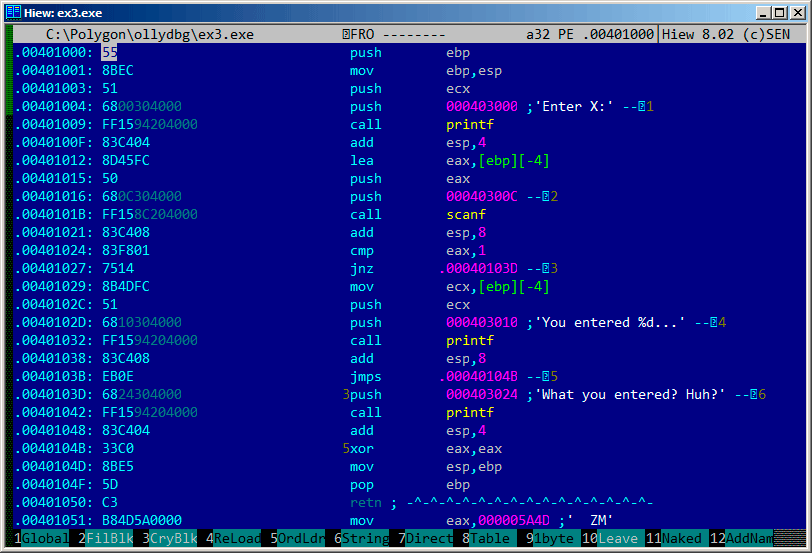
\includegraphics[scale=\FigScale]{patterns/04_scanf/3_checking_retval/hiew_1.png}
\caption{Hiew: \main function}
\label{fig:scanf_ex3_hiew_1}
\end{figure}

Hiew trova le stringhe \ac{ASCIIZ} e le visualizza, cosi' come i nomi delle funzioni importate.

\clearpage
Spostiamo il cursore all'indirizzo \TT{.00401027} (dove si trova l'istruzione \TT{JNZ} che vogliamo bypassare), premiamo F3, e scriviamo \q{9090} (cioe' due \ac{NOP}):

\begin{figure}[H]
\centering
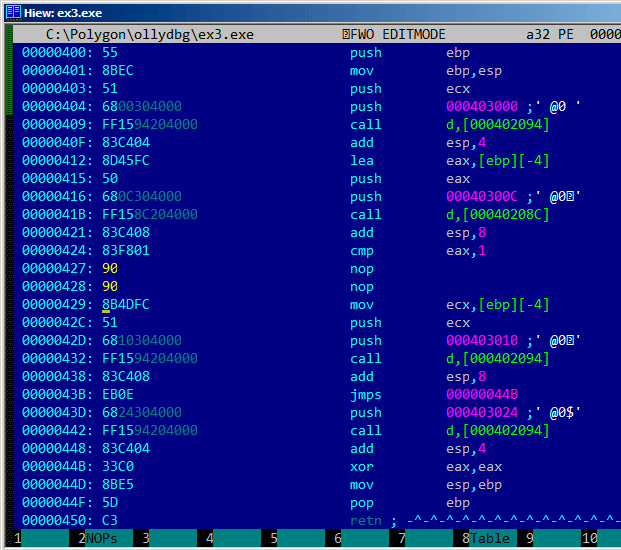
\includegraphics[scale=\FigScale]{patterns/04_scanf/3_checking_retval/hiew_2.png}
\caption{Hiew: replacing \TT{JNZ} with two \ac{NOP}s}
\label{fig:scanf_ex3_hiew_2}
\end{figure}

Premiamo quindi F9 (update). L'eseguibile viene quindi salvato su disco, e si comportera' come vogliamo.

Utilizzare due \ac{NOP} non rappresenta l'approccio esteticamente migliore.
Un altro modo di patchare questa istruzione e' scrivere 0 al secondo byte dell'opcode (\gls{jump offset}), 
in modo che \TT{JNZ} salti sempre alla prossima istruzione.

Potremmo anche fare l'opposto: sostituire il primo byte con \TT{EB} senza toccare il secondo byte (\gls{jump offset}).
Otterremmo un jump non condizionale che e' sempre eseguito.
In questo caso il messaggio di errore sarebbe stampato sempre, a prescindere dall'input.

